\documentclass[a4paper,10pt,oneside]{article}
\usepackage{amsmath,amssymb,epsfig}
\usepackage[T1]{fontenc}
\usepackage{ae,aecompl}
\usepackage{epsfig}
\usepackage{subfigure}
\addtolength{\voffset}{-1cm}
\addtolength{\hoffset}{-1cm}
\setlength{\parindent}{0in}
\addtolength{\textwidth}{1.8cm}
\addtolength{\textheight}{1cm}
\addtolength{\parskip}{.5cm}

\title{Answers for the questions asked during the M/EEG source modeling lecture}

\begin{document}

\maketitle

\noindent \textbf{Question:} The main disadvantages of the Equivalent Current Dipoles approach to source modeling are ...

\noindent \textbf{Answer:}

\begin{itemize}

\item The number of dipoles has to be fixed a priori

\item Finding the location of the dipoles involves a difficult to solve non-linear optimization problem

\item The number of local minima of such non-linear optimization problem increases with the number of dipoles. A \emph{local mininum} is a solution to the optimization problem that is optimal in a local neighborhood. By this we mean that moving the dipoles away a small distance from a local minimum solution leads to an increase of the error between model predictions and observations, therefore suggesting that the optimization process has been completed and we have reached the optimal solution. However, a local minimum is not necessarily the global minimum, i.e. the solution with the minimum achievable error among all possible solutions. See Fig~\ref{fig:local} for more information.

\end{itemize}


\begin{figure}
	\centering
		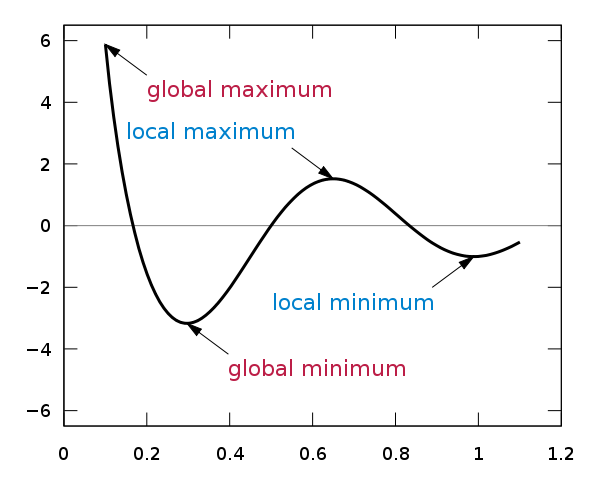
\includegraphics[width=0.75\textwidth]{img/local-minima}
	\caption{Difference between global and local extrema. The vertical line may account for the error between model predictions and observations. Then you may understand the horizontal axis as a parameter that determines the position of the model dipoles. Obviously, finding the best model involves finding the global minimum of the error function (the black line). Note that if you are unlucky enough and the starting point that you choose for the optimization process is located somewhere near a local minimum, you may end the optimization prematurely at a spurious (local) solution rather than at the true solution (the global minimum).}
	\label{fig:local}
\end{figure}

\vspace{1cm}

\noindent \textbf{Question:} The main disadvantages of the distributed approaches to M/EEG source modeling are ...

\noindent \textbf{Answer:}

\begin{itemize}

\item Such approaches require solving a heavily underdetermined inverse problem. As such, there are many model configurations which would fit perfectly our observations and there is no obvious way of choosing among such equally good solutions.

\item The correct definition of the source space is crucial for the success of distributed inverse solvers. Indeed, if the source space does not include the true solution to the inverse problem, any distributed approach is doomed to fail. On the other hand, using a extremely large and dense source space is not wise either. The latter approach will make the inverse problem even more under-determined and will increase the ill-conditioning of the leadfield matrix. Finding the right balance between a too dense and a too sparse source space is far from trivial. Most methods rely on anatomical constraints to approach this problem. One popular solution is to restrict the source space to the cortical mantle, and to enforce that the orientation of the source dipoles is perpendicular to the cortical surface.

\item Defining the boundaries between functionally differentiated sources based on the outcome of distributed inverse solvers is far from trivial, and usually involves a considerable degree of subjectivity.

\end{itemize}


\noindent \textbf{Question:} What is the problem introduced by an ill-conditioned leadfield matrix?

\noindent \textbf{Answer:}

An ill-conditioned leadfield matrix will increase dramatically the noise sensitivity of your inverse solution. See the slides of the lecture on linear algebra fundamentals for an illustration of this effect. 

\noindent \textbf{Question:} What technique can be used to overcome an ill-conditioned leadfield matrix? What is the downside of such technique?

\noindent \textbf{Answer:}

You may partially overcome an ill-conditioned leadfield matrix using \emph{regularization}. Mathematically, regularization involves adding some (arbitrary) terms during leadfield matrix pseudo-inversion. In practice, regularization biases your inverse solver towards a certain sub-set of all valid solutions. Obviously, you will want to use regularization techniques that will introduce a bias towards solutions that seem plausible. In particular, one popular regularization technique involves a bias towards smooth solutions (e.g. the technique used by the LORETA inverse solver). Another (less popular) technique involves a bias towards sparse solutions (e.g. the technique used by the FOCUSS inverse solver).

The downside of regularization is that, by using \emph{a priori} information, we may push the inverse solver towards the solutions that we \emph{expect to find} rather than towards the \emph{most accurate solution}. 


\end{document}